
The main claim holds in every cell tested: training-free per-layer logit-lens uncertainty statistics are class-separable hallucination scores at intermediate depth in all six model $\times$ dataset cells (selection-split corrected AUROC 0.6092--0.7011 against a 0.55 gate), and the best screened intermediate layer beats the same sweep's final-layer entropy readout in every cell. We present the existence grid first, then the structure inside it: the dataset dependence of the depth advantage, the signal-family pattern, the anchor forensics that determined what counts as a baseline, and one finding that contradicted the study's own prediction. Every number below is a selection-split point estimate from a single seed; none is held-out performance.

\subsubsection{5.1 The existence grid}

Table 1 reports the six selected tuples with their within-sweep final-layer baselines. Figure 4 shows the headline comparison --- per-cell best-intermediate AUROC against the 0.55 gate and the final-layer bar; every intermediate bar clears both.

\textbf{Table 1: Selection-split corrected AUROC per cell (single seed, no CIs). Depth margin = best intermediate $-$ within-sweep final-layer entropy.}

\begin{table*}[htbp]
\centering
\resizebox{\dimexpr 2\columnwidth+\columnsep\relax}{!}{%
\begin{tabular}{lllll}
\toprule
Cell & Selected (layer, signal) & Intermediate AUROC & Final-layer entropy AUROC & Depth margin \\
\midrule
LLaMA-2 / TriviaQA & L31, adj. KL & 0.6522 & 0.5928 & +0.059 \\
LLaMA-2 / TruthfulQA & L29, entropy & 0.7011 & 0.6669 & +0.034 \\
Mistral / TriviaQA & L31, max-prob & 0.6092 & 0.5447 & +0.064 \\
Mistral / TruthfulQA & L31, adj. KL & 0.6570 & 0.6048 & +0.052 \\
LLaMA-3 / TriviaQA & L28, entropy & 0.6868 & 0.5566 & +0.130 \\
LLaMA-3 / TruthfulQA & L31, max-prob & 0.6213 & 0.6178 & +0.0035 \\
\bottomrule
\end{tabular}
}
\end{table*}

\begin{figure}[htbp]
\centering
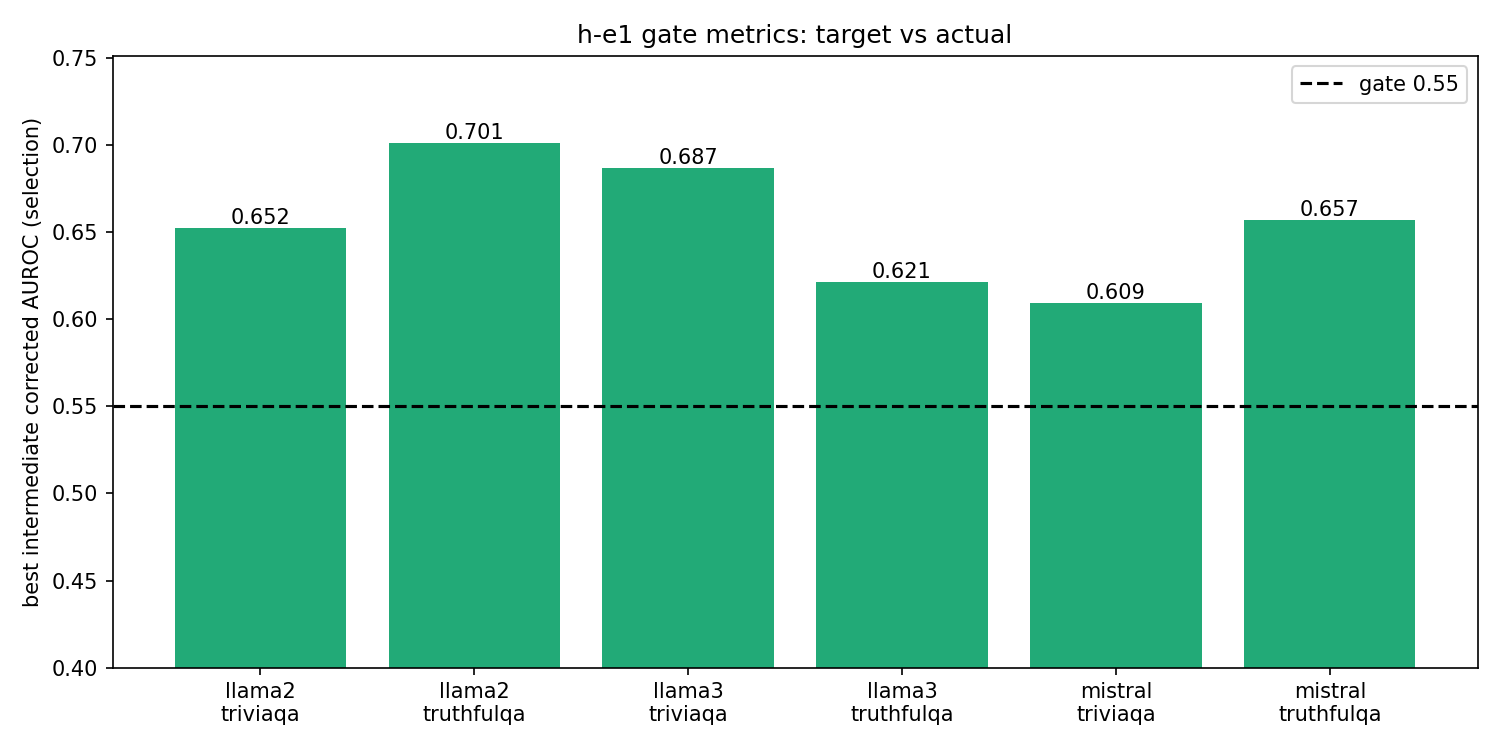
\includegraphics[width=\columnwidth]{figures/gate_metrics_bar.png}
\caption{Figure 4: Existence gate grid --- per-cell best intermediate corrected AUROC vs. the 0.55 gate and the within-sweep final-layer entropy baseline, all six cells.}
\label{fig:gate_metrics_bar}
\end{figure}

The answer to RQ1 is yes in all six cells: the gate clears by +0.059 (Mistral/TriviaQA) to +0.151 (LLaMA-2/TruthfulQA). These are point estimates --- no confidence intervals were computed and no distributional claim is made about the margins; we note only, as a point-estimate comparison, that the thinnest gate margin is an order of magnitude larger than the thinnest depth margin of Section 5.2. The substantive content is universality within scope: the signal appears in a base LLaMA, a base Mistral, and an RLHF-tuned LLaMA-3, under two different labeling protocols --- the intermediate-over-final consensus does extend to statistics that require no probe, at least at the existence tier. The selected layers also concentrate: every winner sits at L28--L31, four of six at L31 itself --- the informative surface is the late-but-not-last band just before output calibration. Figure 5 shows the full layer $\times$ signal grid; the late-band concentration is visible in every cell, not an artifact of the argmax.

\begin{figure}[htbp]
\centering
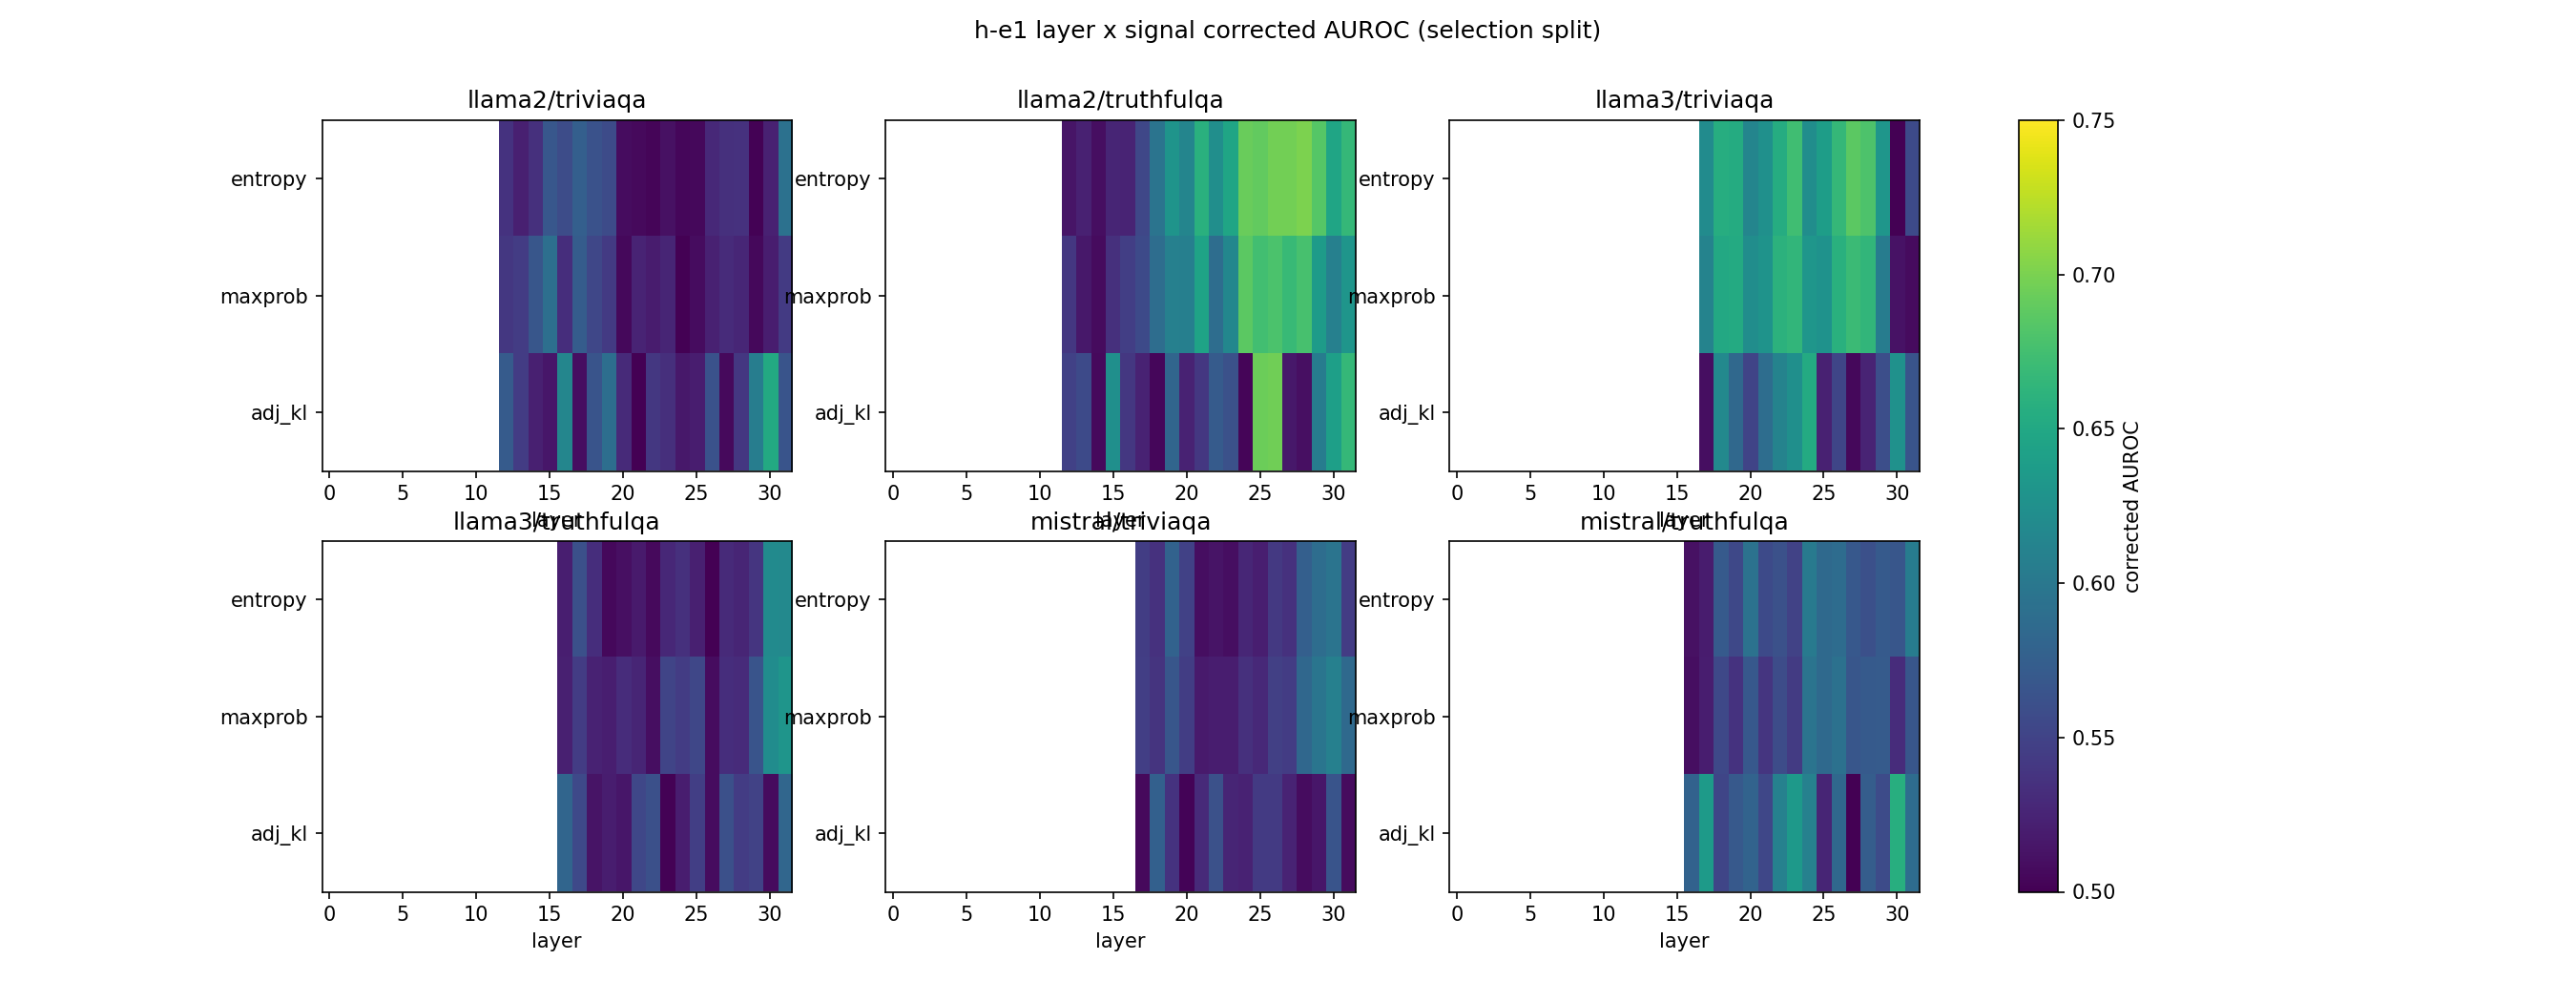
\includegraphics[width=\columnwidth]{figures/auroc_heatmap.png}
\caption{Figure 5: Corrected AUROC across screened layers and signals for all six cells. Informative depth concentrates at L28--L31.}
\label{fig:auroc_heatmap}
\end{figure}

\subsubsection{5.2 The depth advantage is universal in direction, dataset-dependent in size}

RQ2 also resolves 6/6: the best screened intermediate layer beats the within-sweep final-layer entropy readout in every cell. The margins, however, split cleanly by dataset. On TriviaQA they are substantial --- +0.059, +0.064, +0.130 --- while on TruthfulQA they thin to +0.034, +0.052, and +0.0035, because TruthfulQA final layers are already comparatively strong (entropy AUROC 0.6048--0.6669). The thinnest cell warrants an explicit flag: at +0.0035 on 408 selection examples with no confidence interval, LLaMA-3/TruthfulQA's depth advantage is within plausible noise, and it is counted as direction-consistent rather than as evidence. The claim degrades gracefully --- five of six margins exceed 0.03 --- but ''6/6'' is a point-estimate statement, not a statistical one.

The interpretation adds a nuance the mechanism story needs: depth helps most where the final layer is weakest. Where output calibration leaves little separation at L32 (TriviaQA, final-layer AUROC 0.54--0.59), reading before calibration recovers a substantial amount; where the final layer already separates classes (TruthfulQA), there is less to recover. This is consistent with the calibration-suppression reading --- suppression as relative attenuation, not destruction --- while bounding it: whatever suppresses the signal is dataset-dependent. Whether that reflects TruthfulQA's adversarial question design, its similarity-based label protocol, or small-sample variance cannot be decided from this grid; all three explanations remain live.

\subsubsection{5.3 Signal families: belief revision as a detection score}

Adjacent-layer KL --- a statistic with, to our knowledge, no detection-time precedent, previously used only to steer decoding --- is the best signal in two of six cells, with entropy and max-probability each also best in two: an even three-way split. Its strongest showing is the LLaMA-2/TriviaQA cell (Figure 6), where the top three intermediate scores are all adjacent-layer KL: L31 at 0.6522, L17 at 0.6145, L30 at 0.6062. That the winning signal differs across datasets within every model --- and the winning layer within two of the three --- also supports selecting the full (layer, signal, direction) tuple per cell rather than fixing any element a priori.

\begin{figure}[htbp]
\centering
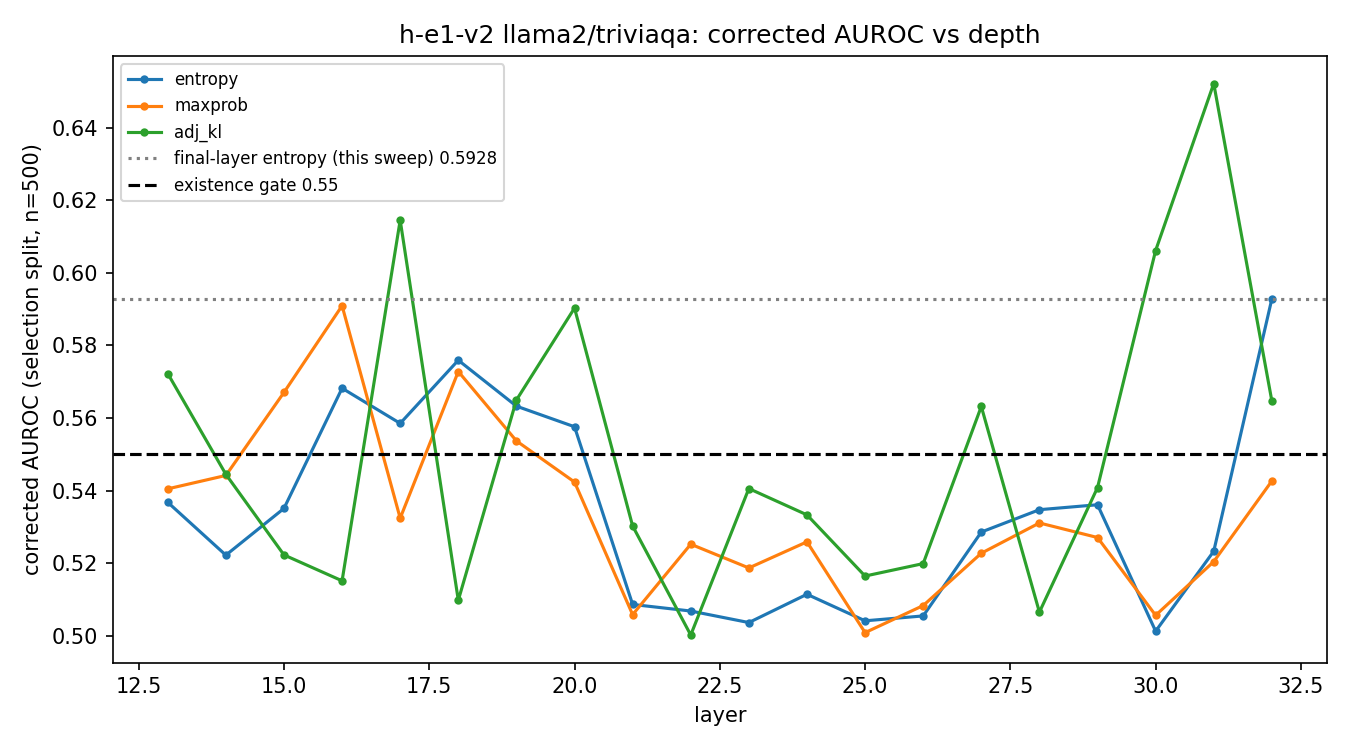
\includegraphics[width=\columnwidth]{figures/auroc_vs_depth_llama2_triviaqa.png}
\caption{Figure 6: AUROC vs. depth for LLaMA-2/TriviaQA --- the three signal curves with the 0.55 gate and final-layer baseline. The top three intermediate scores are all adjacent-layer KL.}
\label{fig:auroc_vs_depth_llama2_triviaqa}
\end{figure}

The implication is that inter-layer belief revision can serve as a detection signal, not just a decoding heuristic --- to our knowledge the first detection-time use of this quantity. What adjacent-layer KL at L31 \textit{measures}, however, is undecidable from these data. Two readings fit: it is an independent ''turbulence'' signal --- persistent belief revision as a distinct facet of unresolved competition --- or it is a meter on the calibration step itself, scoring how much the last layers rewrite the distribution. Both are calibration-adjacent; separating them requires the fusion test and a correlation analysis staged as future work, both computable from the released caches with zero GPU.

\subsubsection{5.4 Anchor forensics: the fate of the baseline this study set out to compare against}

This study was designed around a documented failure: the archived motivating record (Section 1) put final-layer entropy at AUROC 0.5186 on LLaMA-2/TriviaQA. The first experiment version (h-e1) gated on reproducing that number within $\pm 0.03$ --- and the halt gate fired 47 seconds into what was budgeted as a roughly 2.5-hour GPU campaign. The observed value was 0.5928 on the selection split (0.5739 on the full set), a deviation of +0.0742 against a 0.03 tolerance; h-e1's overall gate consequently evaluated to PARTIAL (4 of 6 criteria), with five of six cells intentionally unmeasured by the fail-fast design. A provenance audit found the reference protocol differed in six documented ways: random-sample vs. first-slice data selection, bare vs. templated prompt, substring vs. normalized-alias labels, generation-time vs. teacher-forced lens entropy, bfloat16 vs. fp16, and full-set vs. selection-split evaluation. The anchor was unsatisfiable by construction --- no correct implementation could close a gap created by measuring a different thing. Independent checks support this attribution: the implementation passed its full test suite (35/35), and the donor-label identity check passed 10/10, so the deviation is a property of the reference numbers, not of the code. Figure 7 shows the breach against the tolerance band.

\begin{figure}[htbp]
\centering
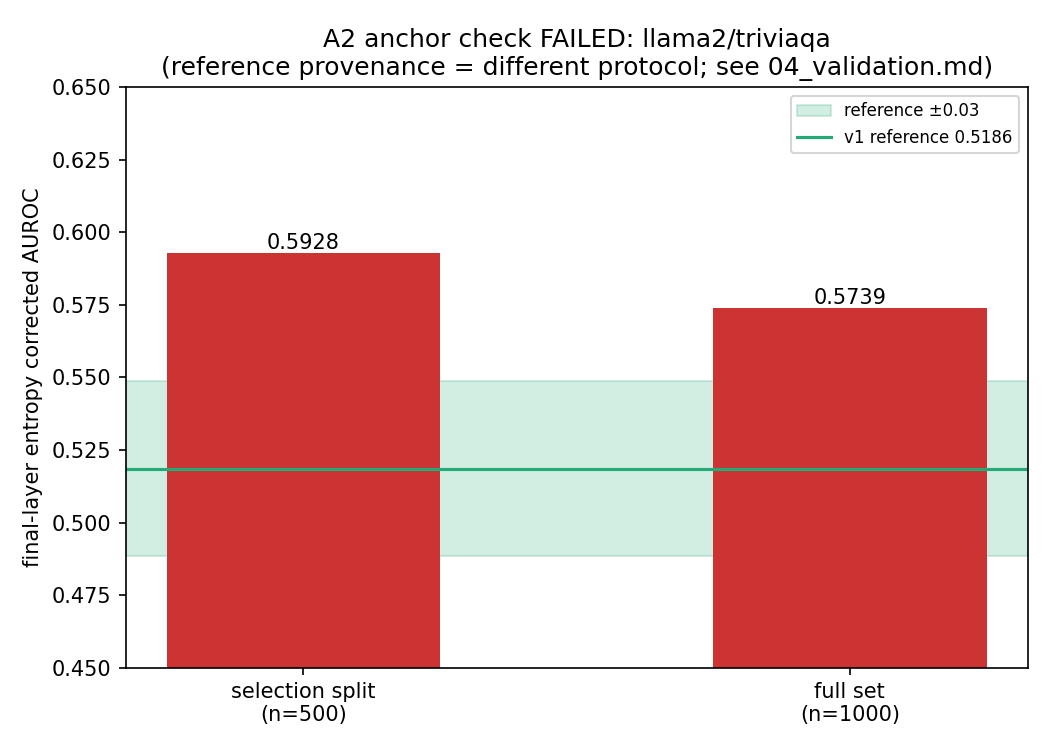
\includegraphics[width=\columnwidth]{figures/h-e1_anchor_check_llama2_triviaqa.png}
\caption{Figure 7: The v1 anchor breach --- observed final-layer entropy AUROC vs. the cross-protocol reference and its $\pm 0.03$ tolerance band on LLaMA-2/TriviaQA.}
\label{fig:h-e1_anchor_check_llama2_triviaqa}
\end{figure}

The redesigned protocol-internal anchor (Section 3.5) then passed all five gate criteria on the full v2 sweep (existence in 6/6 cells, donor identity 10/10, depth-beats-final 6/6, screen health, and the descriptive direction report) with zero spurious halts. The descriptive cross-run check found direction consistent with the motivating record in 4/6 cells, with both inconsistencies on cells that record never code-verified.

This is reported as a result, not an incident report, for two reasons. Scientifically: AUROC magnitudes for weak uncertainty signals are protocol-bound --- six ordinary protocol choices moved the same cell by +0.074 --- so direction transfers across protocols but magnitude does not, and any comparison this paper makes is within-sweep for that reason. Practically: an inexpensive designed halt gate converted a doomed campaign into a 47-second diagnosis, which is a concrete argument for building validity gates into evaluation pipelines before spending compute.

\subsubsection{5.5 A prediction reversed: the depth advantage does not track tuning status as hypothesized}

The mechanism draft predicted that base LLaMA-2, presumed worst-suppressed, would gain most from depth readout, and instruct-tuned LLaMA-3 least. The data reverse this ordering: the largest TriviaQA depth margin (+0.130, Figure 8) belongs to LLaMA-3-8B-Instruct --- the model predicted to need depth least --- with Mistral (+0.064) and LLaMA-2 (+0.059) behind it. A revised hypothesis fits: instruct tuning may \textit{sharpen} final-layer calibration, strengthening suppression rather than weakening it --- still a calibration account, with the opposite tuning polarity. This is stated descriptively only: with a single instruct model in the grid, tuning status is confounded with everything else about the checkpoint, and the base-vs-instruct pair study that could decide it is future work.

\begin{figure}[htbp]
\centering
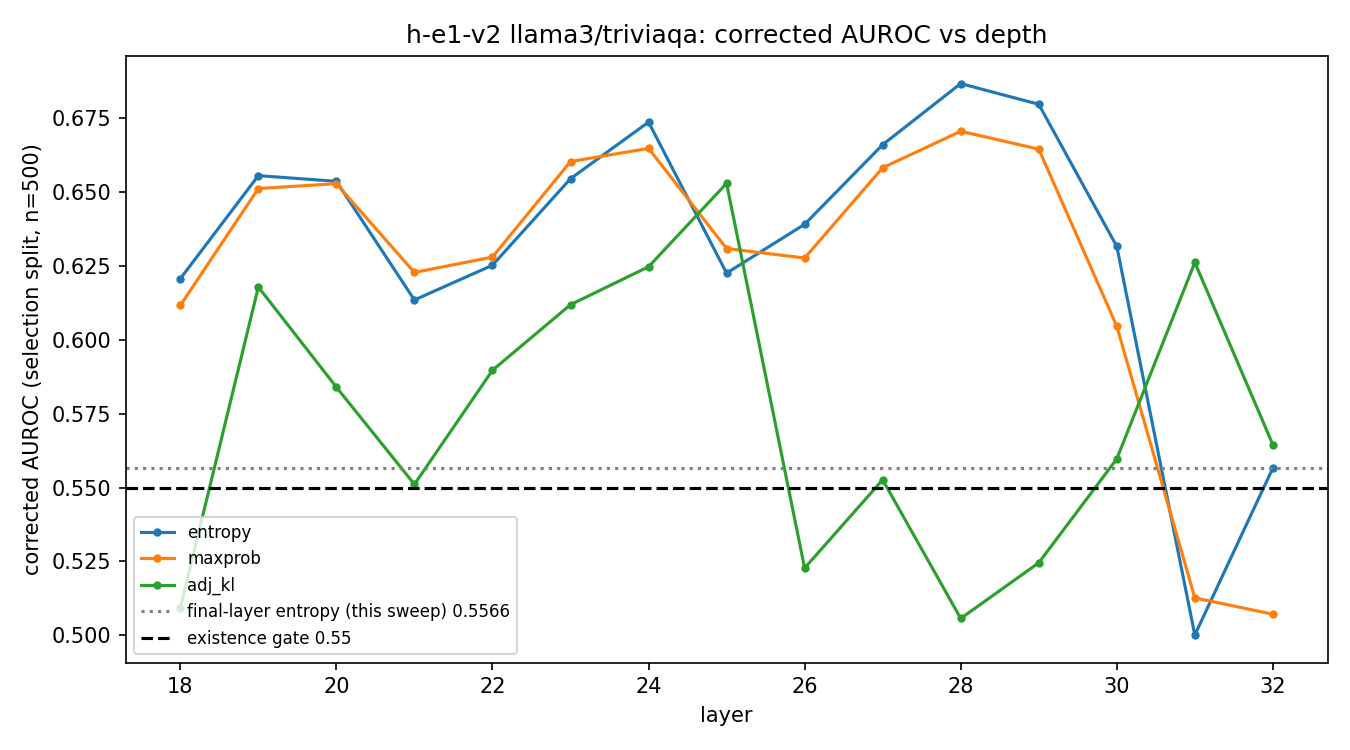
\includegraphics[width=\columnwidth]{figures/auroc_vs_depth_llama3_triviaqa.png}
\caption{Figure 8: AUROC vs. depth for LLaMA-3/TriviaQA --- the largest depth margin in the grid (+0.130), on the model predicted to need depth least.}
\label{fig:auroc_vs_depth_llama3_triviaqa}
\end{figure}

\subsubsection{5.6 What was planned but not measured}

The staged verification design contained four dependent hypotheses beyond the existence tier, none of which was executed: the verification loop's budget was consumed by the h-e1 anchor failure and its v2 re-run, and the loop terminated after the v2 pass with the dependents still queued. Their pre-registered criteria are recorded here because the corresponding predictions are, by design, inconclusive rather than supported:

\begin{itemize}
\item \textbf{Test-split rescue (P1):} frozen tuples achieving test-split AUROC $\geq$ 0.60 on both datasets for LLaMA-2-7B, with a 95\% paired-bootstrap CI on the $\Delta AUROC$ vs. final-layer entropy excluding zero on TriviaQA --- never run.
\item \textbf{Cross-dataset transfer (P2):} the tuple selected on one dataset evaluated on the other's locked test split, within 0.05 AUROC of the natively selected tuple and $\geq$ 0.60, both directions, per model --- never run. Descriptively, best layers cluster at L28--L31 across datasets within each model, which would favor transfer, but the winning signal differs by dataset in four of six cells.
\item \textbf{KL--entropy fusion (P3):} a 2-parameter logistic fusion of the best entropy-family and best KL signals exceeding the best single signal by $\geq$ 0.02 with CI excluding zero in a majority of cells --- never run.
\item \textbf{No-regression guard (P4):} on Mistral and LLaMA-3, selected intermediate AUROC $\geq$ final-layer $-$ 0.02 per dataset on the test split --- never run. On the selection split, the intermediate layer strictly beats the final layer in all four relevant cells, but no test-split evaluation was performed.
\end{itemize}

All four are computable from the released per-example caches with zero GPU; none of their outcomes is claimed here.
